\section{Research Methodology}
\label{sec:methodology}
This section outlines the review protocol, which follows the systematic literature review guidelines of Kitchenham and Charters~\cite{kitchenham2007guidelines}. It covers the research questions, search strategy, eligibility criteria, study selection, and data extraction and synthesis process. PRISMA 2020 is used as a reporting aid for documenting the study-selection flow rather than as the review methodology itself.

\subsection{Research Questions}
\label{sec:research_questions}

To systematically evaluate the technical and operational trade-offs between collaborative SLM--LLM systems and monolithic LLM baselines, the review protocol is structured around the following four core research questions (RQs):

\begin{itemize}
    \item \textbf{RQ1 (Performance):} How does the performance (accuracy/efficacy) of multi-agent SLMs or hybrid architectures (LLM + SLM) compare with that of monolithic LLM baselines in specific reasoning and classification tasks?
    
    \item \textbf{RQ2 (Efficiency):} What is the impact of hybrid and multi-agent architectures on computational efficiency, specifically regarding inference cost, latency, and energy consumption, compared to monolithic LLM baselines or full-LLM inference?
    
    \item \textbf{RQ3 (Orchestration):} What orchestration and routing mechanisms are employed to manage the division of labor between large and small models in collaborative systems?
    
    \item \textbf{RQ4 (Domain Suitability):} In which specific domains (e.g., healthcare, coding, telecommunications, and edge or multimodal settings) do collaborative SLM-centered architectures achieve performance comparable to monolithic LLM baselines, and where do they fail?
\end{itemize}

\subsection{Information Sources and Search Strategy}
\label{sec:search_strategy}

To capture a comprehensive and high-quality corpus of contemporary collaborative language model architectures, the literature search was centered on the Web of Science (WoS) Core Collection, with the final search performed on 8 February 2026. Scopus and the Association for Computing Machinery (ACM) Digital Library were also checked with the same core concepts as coverage validation; deduplicated records from both sources were screened against the eligibility criteria, and no additional studies were identified beyond those already captured by the WoS search. The WoS-centric approach and its implications for coverage are discussed under external validity (Section~\ref{sec:threats}).

The search strategy was systematically developed by extracting the core concepts from the defined research questions and refining the terminology through initial pilot searches in the artificial intelligence (AI) literature. This iterative process helped identify common synonyms and alternate phrasing used in the literature (e.g., ``Compact Model'' for SLMs, or ``Agentic'' for multi-agent systems). To guarantee that every retrieved study examined the intersection of model size, collaborative architectural design, and system evaluation, the final query was structured into four mandatory components and applied to the title, abstract, and keyword fields: \textit{(``Large Language Model*'' OR ``LLM'' OR ``Generative AI'' OR ``Foundation Model*'') AND (``Small Language Model*'' OR ``SLM'' OR ``Compact Model*'' OR ``Lightweight Model*'') AND (``Multi-agent'' OR ``Hybrid'' OR ``Orchestration'' OR ``Routing'' OR ``Ensemble'' OR ``Agentic'') AND (``Performance'' OR ``Accuracy'' OR ``Efficiency'' OR ``Latency'' OR ``Cost'' OR ``Benchmark'')}.

Because the review targets collaborative SLM--LLM systems, all four components were mandatory in the search string. Monolithic LLMs were considered only as baselines reported inside the included studies, not as standalone primary studies.

\subsection{Eligibility Criteria}
\label{sec:eligibility_criteria}

To systematically isolate systems-level engineering research from the broader generative AI literature, retrieved records were evaluated against strict eligibility criteria. A comprehensive breakdown of the inclusion and exclusion parameters applied during the screening phases is presented in Table \ref{tab:eligibility_criteria}.

\begin{table}[!htbp]
    \centering
    \caption{Inclusion and Exclusion Criteria for Study Selection}
    \label{tab:eligibility_criteria}
    \footnotesize
    \setlength{\tabcolsep}{3pt}
    \renewcommand{\arraystretch}{0.94}
    \begin{tabularx}{\linewidth}{@{} >{\raggedright\arraybackslash}p{0.16\linewidth} >{\raggedright\arraybackslash}X >{\raggedright\arraybackslash}X @{}}
        \toprule
        \textbf{Criterion} & \textbf{Include} & \textbf{Exclude} \\
        \midrule
        
        \textbf{Architecture Scope} & 
        Collaborative SLM--LLM systems using routing, retrieval, verification, fallback, or role specialization. & 
        SLM-only papers or monolithic LLM comparisons without a collaborative SLM component; monolithic LLMs were allowed only as baselines inside otherwise eligible studies. \\
        
        \textbf{Model Size and Transparency} &
        Identifiable SLM component with reported or inferable size not exceeding 7B parameters. This upper bound was chosen, rather than a lower one (e.g., 1B--3B), because it marks the practical ceiling for single-accelerator deployment: a 7B-parameter model requires approximately 14~GB of memory at FP16 precision or roughly 4--5~GB once 4-bit quantized, fitting within a single consumer GPU or edge accelerator without multi-device sharding. The threshold is also consistent with the upper range used in related secondary studies on SLM definitions~\cite{slmreview2025prisma,wang2024slmsurvey}, and an upper-bound choice avoids excluding boundary-case models (e.g., Mistral-7B, Qwen2.5-7B) that several included primary studies deploy as their SLM component; closed-box LLMs allowed only as baseline, teacher, or fallback components. &
        Primary architecture depends on closed-box application programming interface (API)-bound models with undisclosed details, or no reproducible SLM component can be identified. \\
        
        \textbf{Topic Focus} & 
        Reports system-level metrics such as performance, latency, memory, cost, or orchestration efficiency. & 
        Focuses only on ethical, sociological, or legal issues without technical benchmarks. \\
        
        \textbf{Data Quality} & 
        Contains empirical results and experimental validation using benchmarks or custom datasets. & 
        Purely theoretical papers or non-empirical narrative surveys. \\
        
        \bottomrule
    \end{tabularx}
\end{table}

\subsection{Study Selection Process}
\label{sec:study_selection}

Following the Kitchenham and Charters review protocol~\cite{kitchenham2007guidelines}, candidate studies were screened against the predefined eligibility criteria and assessed at title, abstract, and full-text stages. The selection flow is summarised in Figure~\ref{fig:prisma} and reported using PRISMA 2020 terminology~\cite{page2021prisma}. The initial search yielded 116 records.

\begin{figure}[!htbp]
\centering
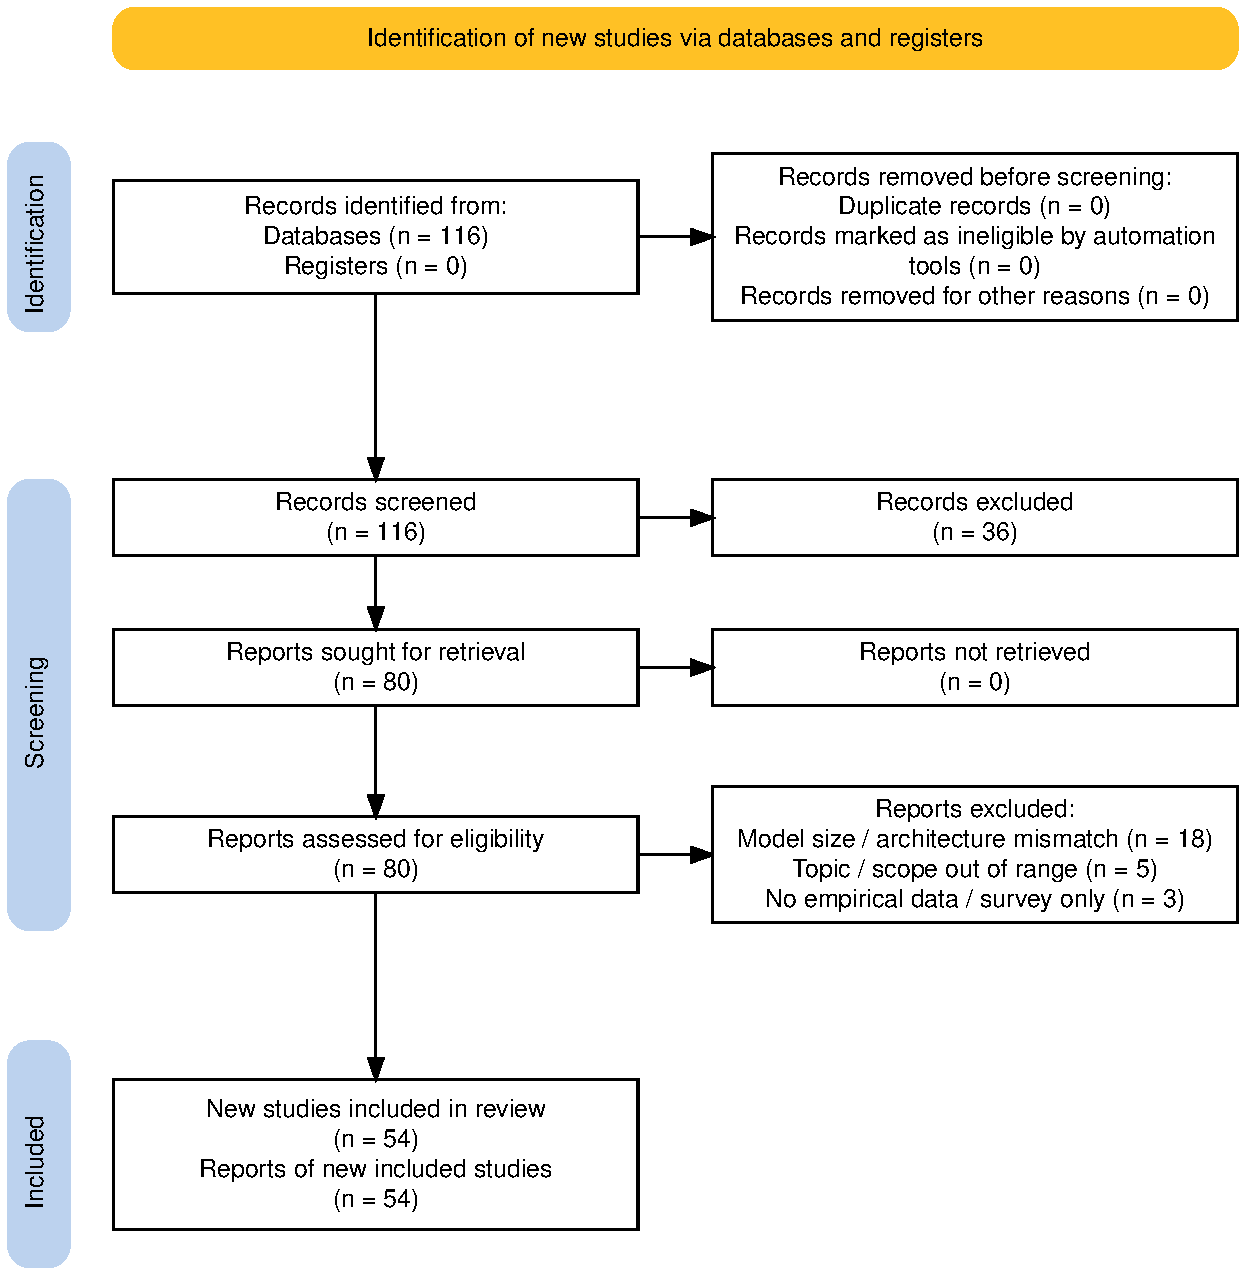
\includegraphics[width=0.75\linewidth]{figures/prisma_flowchart.pdf}
\caption{PRISMA 2020 flow diagram of the study selection process.}
\label{fig:prisma}
\end{figure}

During identification and screening, the title, abstract, and keywords of all records were reviewed manually, excluding 36 records that failed the primary eligibility criteria, including non-technical narrative surveys, extended abstracts without full empirical validation, and studies in unrelated domains. The remaining 80 reports advanced to full-text assessment, where 26 additional records were excluded due to model size or architecture mismatch (n=18), topic or scope mismatch (n=5), or lack of original empirical data or a remaining narrative-survey character (n=3). To improve objectivity, title--abstract screening was performed independently by two reviewers before any discussion; initial pairwise agreement across both screening stages reached 93.1\% (108 of 116 records; 8 records required consensus discussion). Disagreements at both screening stages were resolved through structured consensus discussion, with ties escalated to the academic advisors, resulting in a final corpus of 54 primary studies.

A number of records were identified in preprint form at the time of the search. Because a preprint may be superseded by a peer-reviewed version of record after the search date, every primary study first identified as a preprint was re-checked before submission against Crossref by title and author match rather than by preprint-server metadata alone; the latter is unreliable, since only a minority of the preprint records concerned had the published DOI registered back onto them. All twelve such studies had by then appeared in peer-reviewed venues, and each is cited in this review in its published form, so that every one of the 54 primary studies is traceable to a peer-reviewed record. Three preprints remain in the reference list, all of them background survey citations rather than primary studies. Where publication changed the title, author list, or author order, the published version is authoritative.

\subsection{Data Extraction and Synthesis Strategy}
\label{sec:data_extraction}

To systematically address the research questions, a standardized data extraction protocol was applied to the final corpus of 54 primary studies. For each study, data was extracted into a structured matrix to capture both the functional design of the systems and the empirical evidence used to justify them. 

The extracted fields included the specific SLM and LLM models utilized; the overarching architecture type (e.g., Hybrid, Multi-Agent, Retrieval-Augmented Generation (RAG), Ensemble); orchestration mechanisms; evaluation metrics; baseline models; and quantitative performance indicators (accuracy, latency, cost, and energy). To ensure analytical rigor, each extracted variable was explicitly mapped to one or more of the core Research Questions (RQs). This mapping, together with concise field definitions, is detailed in Table \ref{tab:rq-matrix}.

{\scriptsize
\setlength{\tabcolsep}{2pt}
\renewcommand{\arraystretch}{0.9}
\begin{table}[!htbp]
\centering
\caption{RQ $\times$ data extraction matrix. Check marks indicate direct support; Arch. = architecture, Orchestr. = orchestration, and Base. = baseline.}
\label{tab:rq-matrix}
\begin{tabular}{@{}p{0.12\linewidth}p{0.51\linewidth}>{\centering\arraybackslash}p{0.061\linewidth}>{\centering\arraybackslash}p{0.061\linewidth}>{\centering\arraybackslash}p{0.061\linewidth}>{\centering\arraybackslash}p{0.061\linewidth}@{}}
\toprule
\textbf{Field} & \textbf{Description} & \textbf{RQ1} & \textbf{RQ2} & \textbf{RQ3} & \textbf{RQ4} \\
\midrule
SLM(s) & Specific small language model(s) evaluated, fine-tuned, or deployed. & $\checkmark$ &  &  & $\checkmark$ \\
LLM(s) & Large language model(s) used as a baseline, teacher, or fallback. & $\checkmark$ &  &  & $\checkmark$ \\
Arch. Type & Overall system design (e.g., hybrid, multi-agent, RAG, ensemble). & $\checkmark$ &  &  & $\checkmark$ \\
Orchestr. Method & Coordination mechanism such as routing, decomposition, fusion, or voting. &  &  & $\checkmark$ & $\checkmark$ \\
Agent Count & Number of distinct agents, experts, or role-specific components. &  & $\checkmark$ & $\checkmark$ & $\checkmark$ \\
Task Type & Downstream application, domain, or problem setting evaluated. & $\checkmark$ &  & $\checkmark$ & $\checkmark$ \\
Dataset & Benchmark, open-source corpus, or proprietary data used in evaluation. & $\checkmark$ &  & $\checkmark$ &  \\
Metrics & Evaluation criteria used to assess performance and efficiency. & $\checkmark$ & $\checkmark$ & $\checkmark$ & $\checkmark$ \\
LLM Base. & Standalone performance score of the comparison large model. & $\checkmark$ &  & $\checkmark$ & $\checkmark$ \\
SLM Base. & Standalone performance score of the comparison small model. & $\checkmark$ &  & $\checkmark$ & $\checkmark$ \\
Accuracy & Final performance score achieved by the proposed architecture. & $\checkmark$ &  & $\checkmark$ &  \\
Latency (ms) & Reported inference delay, throughput, or time-to-response. &  & $\checkmark$ & $\checkmark$ & $\checkmark$ \\
Cost (\$) & Reported API cost or computational savings versus full LLM use. &  & $\checkmark$ & $\checkmark$ & $\checkmark$ \\
Energy & Power use, joules-per-token, or carbon-related efficiency metric. &  & $\checkmark$ & $\checkmark$ & $\checkmark$ \\
Findings & Main study takeaway on SLM--LLM collaboration or orchestration. & $\checkmark$ & $\checkmark$ & $\checkmark$ & $\checkmark$ \\
Limits & Reported constraints, failure modes, or deployment bottlenecks. &  & $\checkmark$ & $\checkmark$ &  \\
\bottomrule
\end{tabular}
\end{table}
}

The full comparative analysis table and the comprehensive data extraction spreadsheet are available at \url{https://bit.ly/SLM-LLM-Data-2026}. The Study ID to citation mapping (S1--S54) used throughout this paper is provided in Appendix~\ref{app:study_mapping}, Table~\ref{tab:study_mapping}, for cross-referencing purposes.

Following data extraction, a narrative synthesis approach was utilized. Because the included studies operate across diverse domains (e.g., telecommunications, healthcare, software engineering) and report varying metrics, a purely statistical meta-analysis was not feasible. Instead, studies were grouped by their architectural taxonomy, allowing for a comparative analysis of how different orchestration methods and domain constraints impact the performance and efficiency trade-offs between large and small models.

\noindent\textbf{Data Provenance and Synthesis.}
To formalize the narrative synthesis and ensure evidence traceability, a thematic coding methodology was applied to the extracted data. Studies were grouped not by parameter size, but by their dominant architectural mechanism (e.g., routing, retrieval, or multi-agent debate). Quantitative metrics, including accuracy, latency, and cost, were extracted exactly as reported. Where numerical metrics were absent---such as for the latency overhead in S1---limitations and operational constraints were either extracted verbatim or inferred strictly from conclusions explicitly stated by the primary authors, thereby avoiding post hoc reviewer assumptions. This structured thematic grouping forms the basis of the architectural concept matrix in Table~\ref{tab:concept-matrix}.

\subsection{Synthesis Protocol and Qualitative Coding}
\label{sec:synthesis_protocol}

To ensure that synthesis claims are systematically derived from and traceable to primary evidence, data extraction was followed by a three-pass qualitative coding procedure~\cite{petersen2008systematic}. This procedure standardizes interpretive synthesis decisions across heterogeneous studies and classifies the provenance of extracted statements to distinguish direct evidence from analytical inference.

\textbf{First pass---Architecture and Orchestration Categorization.} Each study was independently coded by two reviewers for (i) primary architecture type: Hybrid, Multi-Agent, Retrieval-Augmented, Ensemble, or Combined; and (ii) dominant orchestration pattern: token-level verification, query-level routing, task decomposition, retrieval augmentation, multimodal fusion, or role specialization. Inter-rater disagreements were resolved through structured discussion, following the same consensus procedure applied during screening (Section~\ref{sec:study_selection}), with escalation to academic advisors for unresolved cases.

\textbf{Second pass---Domain and Metric Coverage Coding.} Each study was classified by primary application domain (Software/Mathematics/Logical Reasoning, Healthcare/Medicine, Telecommunications/Edge/Networking, General NLP/Sentiment/Benchmarking, Specialized Scientific/Spatial, Cybersecurity/Threat Intelligence, or Energy/Resource Optimization) and by metric availability: (a) performance-only; (b) performance plus at least one efficiency metric; or (c) full-metric reporting including accuracy, latency, cost, and energy. This coding produced the distribution statistics reported in Section~\ref{sec:study_characteristics}.

\textbf{Third pass---Performance Outcome and Evidence Provenance Classification.} Each study's primary empirical finding was classified as one of: (a)~outperforms monolithic SLM baseline; (b)~matches monolithic LLM baseline; (c)~outperforms LLM baseline; or (d)~mixed or task-dependent results. Concurrently, each extracted data item was assigned a provenance label:
\begin{itemize}
    \item \textit{Direct numerical extraction}: a quantitative result reproduced verbatim from the primary paper;
    \item \textit{Direct textual extraction}: a qualitative claim or limitation reproduced verbatim or with minor paraphrase, with page reference;
    \item \textit{Analytical synthesis}: a pattern, limitation, or implication derived by the review team from architectural descriptions or indirect evidence in the source paper, where the primary study does not make the statement explicitly.
\end{itemize}
In the supplementary extraction spreadsheet (\url{https://bit.ly/SLM-LLM-Data-2026}), cells derived by analytical synthesis are annotated ``[Synthesized]'' to distinguish them from directly extracted claims. This distinction is particularly relevant for limitation statements: where an author explicitly states that a metric was not measured, the limitation is recorded as a direct textual extraction; where a limitation is inferred by the reviewers from architectural properties not discussed by the authors, it is recorded as an analytical synthesis. For example, in S1 the latency field records ``not reported numerically'' as a direct textual extraction, while the associated limitation note regarding production-time overhead from iterative refinement loops is recorded as an analytical synthesis based on the described pipeline.

Following Webster and Watson~\cite{webstonwatson2002}, synthesis conclusions in Section~\ref{sec:findings} are organized concept-centrically rather than study-by-study: each concept (orchestration pattern, efficiency trade-off, domain constraint) is linked to the studies providing evidence for it via the S1--S54 identifier scheme. Design pattern claims in Section~\ref{sec:implications} were retained as primary implications only when supported by at least four independent primary studies reporting consistent positive outcomes under comparable operational constraints; the supporting study set for each pattern is stated explicitly in that section.
